\documentclass[letterpaper,12pt]{article}
\usepackage{mathtools}
\DeclarePairedDelimiter\abs{\lvert}{\rvert}     %serve per mettere il modulo 
\usepackage{booktabs}
\usepackage{bm}
\usepackage{textcomp}
\usepackage{colortbl}
\usepackage{tabularx}
\usepackage{textcomp}
\usepackage{siunitx}
\usepackage{booktabs}
\usepackage{enumitem}
\usepackage{xcolor}
\usepackage{fancyhdr}
\usepackage{caption}
\usepackage{changepage}
\usepackage{amsmath} 
\usepackage{subcaption}
\usepackage{graphicx}
\usepackage[table]{xcolor} 
\usepackage{colortbl}
\usepackage[margin=1in,letterpaper]{geometry} % decreases margins
\usepackage{cite} % takes care of citations
\usepackage[hidelinks]{hyperref} % adds hyper links inside the generated pdf file
\usepackage{siunitx} % provides the \SI{}{} command for proper typesetting of units
% Define the colors
\definecolor{linkcolor}{RGB}{0, 102, 204}
\definecolor{citecolor}{RGB}{34, 139, 34}
\definecolor{urlcolor}{RGB}{255, 69, 0}
\definecolor{wavelength_406}{RGB}{129, 0, 204}
\definecolor{wavelength_447}{RGB}{0, 53, 255} 
\definecolor{wavelength_402}{RGB}{131, 0, 188}  
\definecolor{wavelength_501}{RGB}{0, 255, 135}
\definecolor{wavelength_440}{RGB}{0, 0, 255}   
\definecolor{wavelength_513}{RGB}{21, 255, 0}   
\definecolor{wavelength_nan}{RGB}{210,210,210} 
\definecolor{wavelength_540}{RGB}{129, 255, 0}  
\definecolor{wavelength_458}{RGB}{0, 113, 255}  
\definecolor{wavelength_568}{RGB}{219, 255, 0}
\definecolor{wavelength_587}{RGB}{255, 233, 0} 
\definecolor{wavelength_585}{RGB}{255, 239, 0} 
\definecolor{wavelength_472}{RGB}{0, 178, 255}
\definecolor{wavelength_667}{RGB}{235, 0, 0}  
\definecolor{wavelength_676}{RGB}{227, 0, 0}  
\definecolor{wavelength_640}{RGB}{255, 33, 0}  
\definecolor{wavelength_696}{RGB}{209, 0, 0}
\definecolor{wavelength_449}{RGB}{0, 65, 255}
\definecolor{wavelength_503}{RGB}{0, 255, 110}
\definecolor{wavelength_581}{RGB}{255, 252, 0}


% Setup hyperref
\hypersetup{
    colorlinks=false, % colored links
    linkcolor=linkcolor, % color for internal links
    citecolor=citecolor, % color for citations
    urlcolor=urlcolor, % color for URLs
}
\fancypagestyle{logoheader}{
    \fancyhf{}
    \fancyhead[L]{
\includegraphics[width = 3cm]{infn-art-science-universita-degli-studi-di-milano-bicocca-maintainer-universita-studi-milano-bicocca.png}}
    \renewcommand{\headrulewidth}{0pt}
    }
\usepackage{blindtext}
\graphicspath{{immagini/}}
%Required for inserting images
%++++++++++++++++++++++++++++++++++++++++
%Margini 


\begin{document}


\title{{\small Università degli studi Milano-Bicocca  Dipartimento di Fisica - Laboratorio II }\\
	Esperienza Ottica - Interferometro}
\author{F. Ballo, S. Franceschina, S. Dolci - Gruppo T1 39}
\date{\today}
\maketitle
\thispagestyle{logoheader}


\begin{abstract}
	Nella seguente relazione vengono presentati i risultati ottenuti dalla sesta esperienza del corso di 
    Laboratorio II riguardante l'analisi di fenomeni ottici.
    L'obiettivo di questa esperienza è quello di riprodurre due esperimenti di interferometria: Fabri-Perot e Michelson.
    Per ciascuno di questi setup riprodotti in laboratorio lo scopo è quello di verificare certe relazioni, che occorrono
    nel momento in cui raggi luminosi interferiscono tra loro, dalle quali è possibile ricavare informazioni utili come 
    la lunghezza d'onda della sorgente.
	\begin{adjustwidth}{-1cm}{-1cm}
	\end{adjustwidth}
\end{abstract}
\tableofcontents
\newpage

\section{Configurazione setup esperienza}
Per le misure di questa esperienza abbiamo utilizzato:

\begin{itemize}
    \item Un interferometro di precisione PASCO scientific Modello OS-9255A/OS-9258A , \href{https://www.pasco.com/products/lab-apparatus/light-and-optics/advanced-optics/os-9255}{[link]}
    \item Sorgente: laser monocromatico He-Ne con lunghezza d'onda $\lambda = \SI{632.8}{\nano\meter}$.
    \item Lente divergente: lente da 18mm.
    \item Specchi compresi nella dotazione PASCO
\end{itemize}


\section{Fabry-Perot}
La prima parte dell'esperienza consiste nella verifica della legge che descrive
i massimi di interferenza, visibili quando due sorgenti si sommano in fase. 
Per farlo abbiamo montato l'interferometro in configurazione Fabry-Perot:

\begin{figure}[ht]
    \centering
    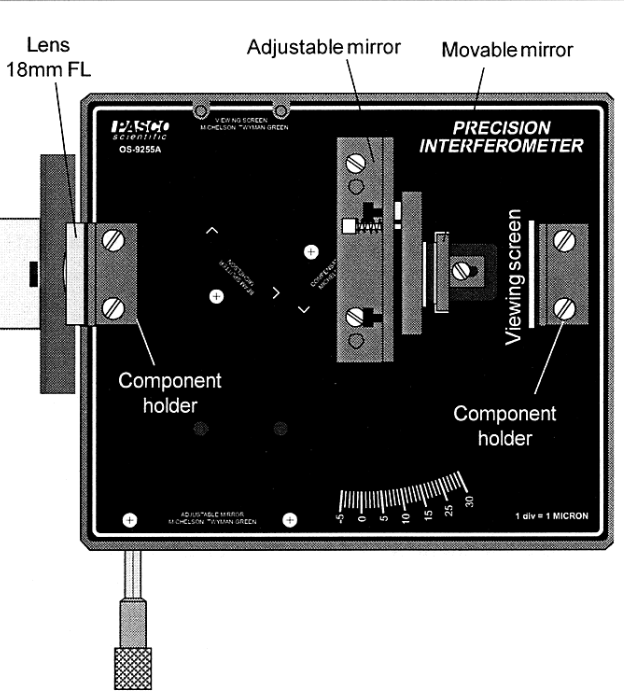
\includegraphics[width=0.4\textwidth]{InterferometroFabry.png}
    \caption{Configurazione Fabry-Perot.}
    \label{fig:fabry-perot config}
\end{figure}

La luce del fascio laser incide contro una lente divergente e entra nella cavità di Fabry-Perot, ovvero due specchi semiriflettenti 
distanziati $d$. Le riflessioni successive tra i due specchi formano la figura di interferenza sullo schermo, posto
a circa un metro di distanza. \\ 
È interessante notare come, per ricavare le relazioni che verranno utilizzate per descrivere il fenomeno, si 
introduca l'ipotesi che i raggi luminosi siano paralleli tra di loro nell'ingresso della cavità, nonostante la 
presenza di una lente divergente. Abbiamo motivato questa ipotesi osservando che la lente divergente è posta
molto vicina alla cavità, e quindi la divergenza dei raggi luminosi è trascurabile. Non si può dire lo stesso per 
quanto riguarda i raggi che incidono sullo schermo, essi infatti sono considerati divergenti perchè la distanza tra
schermo e specchio è significativa.\\
Un'altra osservazione importante riguarda gli angoli delle frange di interferenza. 
Per l'angolo $\theta$, quello riportato in figura \ref{fig:fabry_perot_scheda}, 
abbiamo posto il vertice nel fuoco della lente divergente (18mm avanti) e misurato la distanza tra tale fuoco e lo schermo. 
In questo modo, misurando in seguito la distanza tra il centro della figura di interferenza e la frangia, 
è possibile calcolare l'angolo $\theta$ come l'arcotangente del rapporto tra le due distanze. In ogni caso, tali 
considerazioni sono state rilevanti solo per questa prima parte dell'esperienza, in cui era richiesto di verificare 
la legge \ref{eq:fabry_perot} confrontando i valori di angoli attesi con quelli misurati. Per tutte le altre esperienze 
abbiamo potuto considerare $\theta \approx 0$ e quindi $\cos(\theta) \approx 1$ poichè lo schermo si trova 
a una grande distanza dalla sorgente puntiforme.
\begin{figure}[h!]
    \centering
    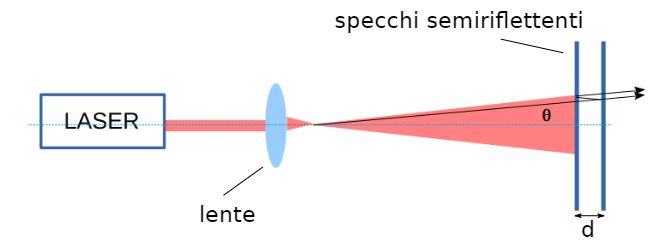
\includegraphics[width=0.4\textwidth]{fabry_perot_config.JPG}
    \caption{Configurazione Fabry-Perot.}
    \label{fig:fabry_perot_scheda}
\end{figure}

\subsection{Verifica della legge di interferenza}

In questa prima parte dell'esperienza abbiamo cercato di verificare
la seguente legge di interferenza, che descrive quando i due raggi luminosi interferiscono in fase:

\begin{equation}
    \delta_r \frac{\lambda}{2 \pi} + 2d \cos(\theta) = N \lambda
    \label{eq:fabry_perot}
\end{equation}

$d$ è la distanza tra i due specchi, $\delta_r$ rappresenta lo sfasamento , $\theta$ è l'angolo di incidenza della luce, $N$ è l'ordine di interferenza e $\lambda$ 
è la lunghezza d'onda del laser sorgente. \\
Per verificarla abbiamo deciso di invertire la relazione in modo da evidenzare la dipendenza di $\cos(\theta)$ dalle
altre variabili, ricavando la relazione \ref{eq:fabry_perot_cos}:

\begin{equation}
    \cos(\theta) = \frac{N \lambda}{2d} - \frac{\delta_r \lambda}{4 d \pi}
    \label{eq:fabry_perot_cos}
\end{equation}
Dopo aver verificato le opportune calibrazioni del laser, delle lenti e dello specchio,
abbiamo misurato il diametro dei cerchi di interferenza con un calibro e calcolato così il coseno dell'angolo $\theta$.\\

\subsection{Analisi Dati legge di interferenza}
Di seguito riportiamo i dati raccolti in laboratorio; la distanza dello schermo dalla sorgente è pari a $D = 1.37 \pm0.01 m$, assumendo come punto sorgente il fuoco della lente 
(18mm). Successivamente per la verifica del modello abbiamo eseguito un'interpolazione con la legge \ref{eq:fabry_perot_cos}, mantenendo come 
parametri liberi $\delta_r$ e $d$.\\
Abbiamo ripetuto tale misura per quattro volte, variando d, al fine di poter verificare in più configurazioni la 
legge \ref{eq:fabry_perot}.\\
Riportiamo i grafici dei fit ottenuti per ciascuna delle misurazioni in figura \ref{fig:verifica_fabry_perot}:

%Da discutere gli errori (anche in relazione ai valori di chi quadro ottenuti)

\begin{figure}[h!]
    \centering
    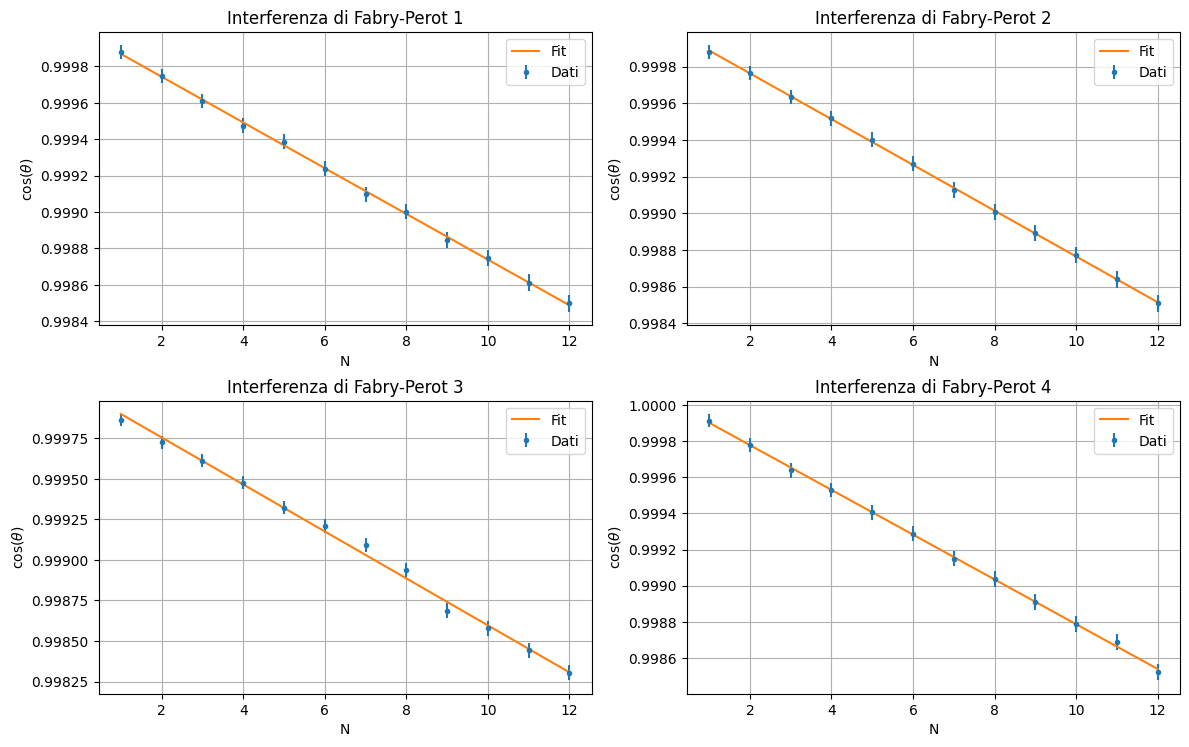
\includegraphics[width=1\textwidth]{verifica_fabry_perot.png}
    \caption{Interpolazioni della legge \ref{eq:fabry_perot_cos}.}
    \label{fig:verifica_fabry_perot}
\end{figure}

Nella tabella \ref{tab:dati_interpolazioni_FP} riportiamo i valori ottenuti per i parametri $\delta_r$ e $d$ 
con i relativi errori, insieme ai valori del $\tilde{\chi}^2$ e p-value trovati dalle interpolazioni.

%Da discutere le unità di misura dei parametri.

\begin{table}[h!]
    \centering
    \begin{tabular}{|c|c|c|  |c|c|c|}
    \hline
    \multicolumn{3}{|c||}{\textbf{Interpolazione 1}} & \multicolumn{3}{c|}{\textbf{Interpolazione 2}} \\
    \hline
    \textbf{Parametro} & \textbf{Valore} & \textbf{Errore} & \textbf{Parametro} & \textbf{Valore} & \textbf{Errore} \\
    \hline
    \text{d} & 0.00252 & 4.82e-07 & \text{d} & 0.00254 & 4.83e-07 \\
    \textbf{$\delta_r$} & 5.01e+04 & 9.56 & \textbf{$\delta_r$} & 5.04e+04 & 9.58 \\
    \hline
    \textbf{$\tilde{\chi}^2$} & 07 & \textbf{p-value :} 1 & \textbf{$\tilde{\chi}^2$} & 0.0398 & \textbf{p-value :} 1 \\
    \hline
    \addlinespace[10pt]
    \hline
    \multicolumn{3}{|c||}{\textbf{Interpolazione 3}} & \multicolumn{3}{c|}{\textbf{Interpolazione 4}} \\
    \hline
    \textbf{Parametro} & \textbf{Valore} & \textbf{Errore} & \textbf{Parametro} & \textbf{Valore} & \textbf{Errore} \\
    \hline
    \text{d} & 0.00219 & 4.22e-07 & \text{d} & 0.00255 & 4.84e-07 \\
    \textbf{$\delta_r$} & 4.34e+04 & 8.36 & \textbf{$\delta_r$} & 5.06e+04 & 9.60 \\
    \textbf{$\tilde{\chi}^2$} & 0.75 & \textbf{p-value :} 0.678 & \textbf{$\tilde{\chi}^2$} & 0.0756 & \textbf{p-value :} 1 \\
    \hline
    \end{tabular}
    \caption{Dati, deviazioni e test $\tilde{\chi}^2$ con p-value, suddivisi per interpolazione.}
    \label{tab:dati_interpolazioni_FP}
    \end{table}

\subsection{Calibrazione micrometro - Frange}
L'interferometro in configurazione Fabry-Perot è dotato di un micrometro che permette 
di variare la distanza tra i due specchi $\Delta d$.
Quando questa $\Delta d$ varia, varia anche il cammino ottico dei raggi luminosi e quindi la posizione delle frange di interferenza.
La legge che lega questo spostamento è la seguente:
    \begin{equation}
        \Delta d = \frac{\Delta N \cdot \lambda}{2 \cdot \cos(\theta)}
        \label{eq:micrometro}
    \end{equation}

Misurando quante frange scorrono sullo schermo è possibile risalire a una misura di maggior precisione
del $\Delta d$ e quindi calibrare il micrometro.\\
Dopo aver registrato una posizione di partenza inziale dello specchio abbiamo scelto $\Delta d_\text{nonio} = 20\text{\SIUnitSymbolMicro m}$ come passo del nonio,
 il coseno dell'angolo $\theta$ approssimato a circa 1, dato che assumiamo incidenza normale.
Infine abbiamo ripetuto la misura più volte, sempre ripartendo
dalle stessa posizione iniziale cercando così di ridurre l'errore 
statistico e ottenendo una media per la distanza.


%Riguardiamo gli errori
\subsection{Analisi Dati calibrazione micrometro}
Riportiamo in seguito i dati ottenuti dalle misurazioni:


Per la stima della distanza, riportiamo il valor medio e l'errore standard 
$$\Delta d_\text{mis} = (19.41 \pm0.11)\ \text{\SIUnitSymbolMicro m} $$
Per questi calcoli abbiamo utilizzato come valore tabulato la lunghezza d'onda del laser He-Ne $\lambda = \SI{632.8}{\nano\meter}$ \href{https://www.pasco.com/products/lab-apparatus/light-and-optics/advanced-optics/os-9255}{[link]}.
Abbiamo inoltre verificato che anche utilizzando $\lambda_\text{aria} = \frac{\lambda_0}{n_\text{aria}}$ dove $n_\text{aria} = 1,0003$ 
è l'indice di rifrazione dell'aria, la precisione della misura non cambia.\\
Mostrare questo fatto numericamente

\subsection{Conclusioni Fabry-Perot}

\newpage
\section{Interferometro Michelson}
Nella seconda parte dell'esperienza abbiamo montato l'interferometro in configurazione Michelson, prima per verificare 
la calibrazione del micrometro (e confrontarla con Fabry-Perot), poi per effettuare altre misure sull'indice di rifrazione
dell'aria e del vetro.
\begin{figure}[h]
    \centering
    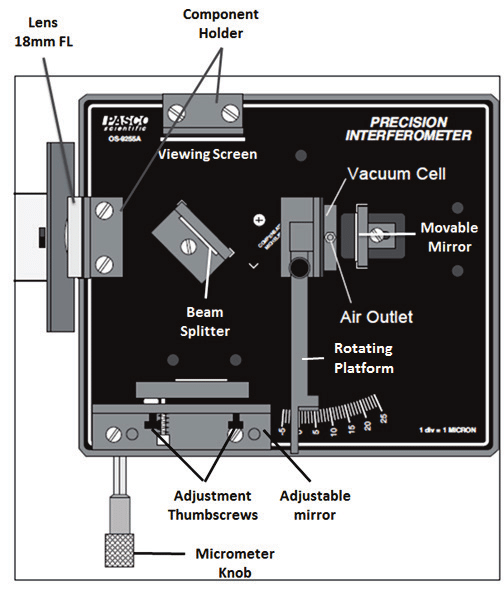
\includegraphics[width=0.4\textwidth]{Michelson_aria.png}
    \caption{Configurazione Michelson.}
    \label{fig:michelson config}
\end{figure}

\subsection{Verifica calibrazione micrometro}
Per la calibrazione del micrometro abbiamo seguito lo stesso procedimento utilizzato per Fabry-Perot, 
utilizzando la  \ref{eq:micrometro} per calcolare la distanza $\Delta d$ percorsa dallo specchio mobile. Abbiamo ripetuto
la misura per quattro volte, spostando con un passo di $20 \text{\SIUnitSymbolMicro m}$, (valore segnato 
dal nonio). Riportiamo in tabella \ref{tab:calibrazione_micrometro_michelson} i risultati. Come valore ottenuto
abbiamo deciso di considerare la media delle misure effettuate, e per errore la loro deviazione standard, in quanto 
misure non dotate di errore poichè ricavate a partire da N e $\lambda$:
$$\Delta d_\text{mis} = (19.36 \pm0.10)\ \text{\SIUnitSymbolMicro m} $$
L'errore sul valore medio è stato calcolato pesando 
gli errori delle singole misure, con la formula \ref{eq:errore_valore_medio}:
\begin{equation}
    %\sigma_{\bar{x}} = \frac{1}{N} \sqrt{\sum_{i=1}^{N} (\sigma_i)^2}
    \sigma_{\bar{x}} = \sqrt{\frac{\sum_{i=1}^{N} (\sigma_i)^2}{N}}
    \label{eq:errore_valore_medio}
\end{equation}


\subsection{Confronto tra due metodi di calibrazione}

Abbiamo confrontato i valori ottenuti per la calibrazione del micrometro con i due diversi setup, Fabry-Perot e Michelson:
\begin{itemize}
    \item[-] Fabry-Perot: $\Delta d_\text{mis} = (19.41 \pm0.11)\ \text{\SIUnitSymbolMicro m} $
    \item[-] Michelson: $\Delta d_\text{mis} = (19.36 \pm0.10)\ \text{\SIUnitSymbolMicro m} $
\end{itemize}

Entrambi i metodi di misura in teoria raggiungono la stessa precisione, essendo entrambi basati sulla stessa legge di interferenza.
Tuttavia i valori ottenuti per la distanza $\Delta d$ sono leggermente diversi, e questo può essere dovuto a diversi fattori.
E' risaputo che l'interferometro Fabry-Perot sia il metodo che permette di raggiungere una risoluzione spettrale maggiore (frange più nitide e distinte), tuttavia questo risulta più utile nelle misure di lunghezze d'onda.
Ci aspettiamo invece che Michelson sia il metodo più preciso per la misura della distanza $\Delta d$ , sia per quanto riguarda il setup e l'allineamento degli specchi (Fabry-Perot era molto più sensibile a vibrazioni del piano di lavoro)
sia per la maggiore distanza tra specchio e schermo, il che dovrebbe ridurre l'errore di misura.\\


\newpage

\subsection{Misura indice rifrazione aria}
In questa parte dell'esperienza abbiamo utilizzato l'interferometro in configurazione di Michelson per misurare l'indice di rifrazione 
dell'aria, sfruttando la sua dipendenza lineare dalla pressione. La configurazione dell'apparato ricalca quella della figura \ref{fig:michelson config}, 
con l'unica differenza il fatto che è stata inserita una cella a vuoto in uno dei bracci dell'interferometro.\\
Al variare della pressione dell'aria all'interno della cella, l'indice di rifrazione dell'aria cambia; come conseguenza, è possibile
osservare un cambiamento nel numero di frange di interferenza che scorrono sul muro.\\
Ci siamo serviti della formula \ref{eq:indice_rifrazione_aria} per risalire all'indice di rifrazione dell'aria :
\begin{align}
    n &= 1 + m \cdot P \\
    m &=  \frac{\Delta N \lambda }{2 d (P_i - P_f)}
    \label{eq:indice_rifrazione_aria}
\end{align}

Laddove $P_i$ e $P_f$ sono le pressioni iniziale e finale ($P_i = \SI{101.325}{\kilo\pascal}$), $\Delta N$ 
è il numero di frange contate, $d = \SI{0.03 \pm 0}{m}$ la larghezza della cella a vuoto e $\lambda$ è la 
lunghezza d'onda del laser.\\
Come procedura di misura abbiamo fatto variare la pressione nella cella a vuoto e contato il numero di frange che scorrevano
sul muro. Abbiamo ripetuto la misura quattro volte, variando la pressione finale, e contando le 
frange di interferenza. Riportiamo in tabella \ref{tab:indice_rifrazione_aria_dati} i dati raccolti e in tabella 
\ref{tab:indice_rifrazione_aria} i valori ottenuti per l'indice di rifrazione dell'aria. 


Gli errori sui singoli valori dell'indice di rifrazione sono stati calcolati con la formula di propagazione degli errori,
a partire dalle relazioni \eqref{eq:indice_rifrazione_aria}, in cui $P_f$ ha come errore la sensibilità del manometro 
($\SI{2}{\kilo\pascal}$). L'errore sul valore medio è stato calcolato pesando gli errori delle singole misure, con la 
formula \eqref{eq:errore_valore_medio}.

Dopo aver calcolato il valore dell'indice di rifrazione dell'aria per le pressioni misurate, abbiamo proceduto eseguendo un fit tramite
un modello lineare per stimare il valore della costante $m$ e il suo errore. Il risultato del fit è riportato in figura \ref{fig:m_aria};
il valore ottenuto è:
$$m = (2.484 ± 0.033)\cdot 10^{-9} \ \text{Pa}^{-1}$$

\begin{figure}[h!]
    \centering
    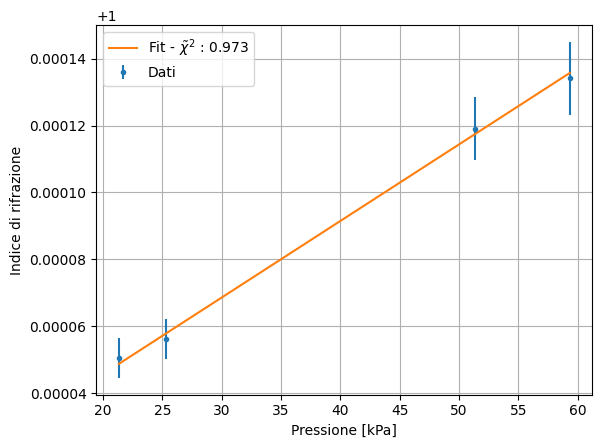
\includegraphics[width=0.6\textwidth]{fit_m_aria.png}
    \caption{Fit lineare per l'indice di rifrazione dell'aria.}
    \label{fig:m_aria}
\end{figure}

Operando un test di compatibilità con il valore atteso, pari a $m = 2.887 \cdot 10^{-9}$ Pa, otteniamo un valore del
t-test pari a $t \approx 11$, molto lontano dal valore desiderato di 1.
Sospettiamo alla base di questa discrepanza ci sia un errore sistematico, probabilmente dovuto a un'errata calibrazione
della cella a vuoto.
Un altra fonte di errore potrebbe essere un incorretto conteggio o un'errata interpretazione delle frange stesse.\\


\subsection{Misura indice rifrazione vetro}
Sempre mantenendo la configurazione Michelson, abbiamo montato un supporto con una lastra di vetro (spessore $d= 5\text{mm}$), come rappresentato in figura \ref{fig:michelson_vetro},
al fine di ricavarne l'indice di rifrazione.
\begin{figure}[h!]
    \centering
    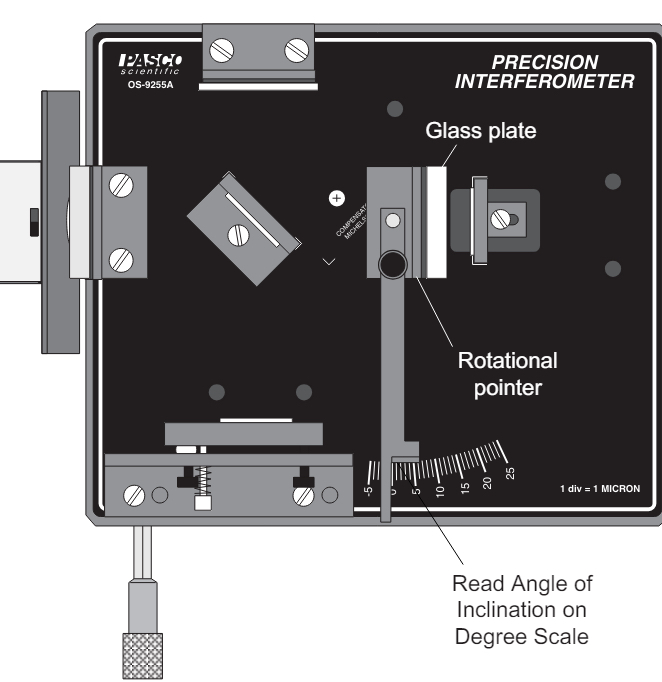
\includegraphics[width=0.4\textwidth]{Michelson_vetro.png}
    \caption{Configurazione Michelson con vetro.}
    \label{fig:michelson_vetro}
\end{figure}

 Servendoci di un rotational pointer è possibile
aumentare o diminuire l'angolo di incidenza del raggio sulla lastra, allungando o accorciando il cammino ottico 
del raggio nel mezzo, di conseguenza, similmente a quanto fatto prima, possiamo contare il numero di frange $\Delta N$ che scorre 
al variare dell'angolo $\theta$, il tutto è governato dalla legge \eqref{eq:fringe_count}:
\begin{equation}
2 \cdot d \cdot (D_i - D_f) = \Delta N \cdot \lambda
\label{eq:fringe_count}
\end{equation}

Dove D e D' sono le distanze percorse in aria, mentre d e d' percorse in vetro:
\begin{itemize}
    \item[-] $D_i = D \cdot n_\text{aria} + d \cdot n_\text{vetro}$
    \item[-] $D_f = D' \cdot n_\text{aria} + d' \cdot n_\text{vetro}$
\end{itemize} 

La formula per ricavare l'indice di rifrazione del vetro è dunque la seguente:
\begin{equation}
    n_\text{vetro} = \frac{(2d -\Delta N \lambda)(1-\cos(\theta))}{2d (1-\cos(\theta)) - \Delta N \lambda}
    \label{eq:indice_rifrazione_vetro}
\end{equation}

Abbiamo ripetuto la misura quattro volte, partendo sempre dal minimo cammino ottico come posizione iniziale
e raggiungendo vari diversi angoli finali. Riportiamo in tabella \ref{tab:calibrazione_micrometro_michelson} i risultati ottenuti:


Gli indici di rifrazione del vetro ottenuti sono stati calcolati con la formula \ref{eq:indice_rifrazione_vetro} e le incertezze
con la formula per la propagazione degli errori. Il valore medio ottenuto per l'indice di rifrazione del vetro è:
$$ n_\text{vetro} = 1.70 \pm 0.05$$


\subsection{Misura lunghezza d'onda con righello reticolo}

Lo scopo di questa sezione è misurare la lunghezza d'onda del laser utilizzato in laboratorio, tramite l'utilizzo 
di un righello, le cui tacche agiscono da reticolo. Riportiamo in figura \ref{Righello_config} la configurazione
che abbiamo seguito per effettuare le misure.

\begin{figure}[h!]
    \centering
    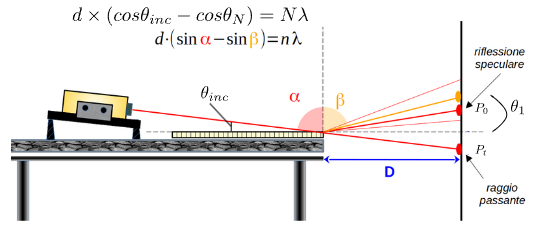
\includegraphics[width=0.4\textwidth]{Righello_config.png}
    \caption{Configurazione righello reticolo.}
    \label{fig:Righello_config}
\end{figure}

In particolare, la distanza tra le tacche è di $d = \SI{1}{\milli\meter}$, e la distanza tra il righello e lo 
schermo è di $D = \SI{1.03}{\meter}$.\\
La formula che lega la lunghezza d'onda alla distanza tra le frange di interferenza è la seguente:

\begin{equation}
    \lambda = \frac{d (\cos(\theta_{inc})-\cos(\theta_N))}{N}
    \label{eq:lunghezza_onda}
\end{equation}

Dove abbiamo indicato con $d$ la distanza tra le tacche del righello, N l'ordine di interferenza, $\theta_{inc}$ 
l'angolo di incidenza del raggio luminoso(abbiamo inclinato il laser), $\theta_N$ l'angolo tra la normale allo schermo e l'N-esimo massimo di 
interferenza.\\

Abbiamo osservato sullo schermo due punti più luminosi, il primo corrispondente al massimo di riflessione dell'ordine $N = 0$ e il secondo al raggio passante.
Oltre a questi due punti sono comparsi altri N-massimi di interferenza , dai quali è possibile ricavare allo stesso modo la relazione tra l'ordine N e l'angolo corrispondente.

Riportiamo in seguito i risultati ottenuti per queste misure:


Il valor medio e la deviazione standard ottenuti per la lunghezza d'onda del laser è 

$$ \lambda_\text{mis1}= (666 \pm 14) \text{nm}$$
$$ \lambda_\text{mis2}= (640 \pm 19) \text{nm}$$



Per rispondere alla domanda "Cosa cambia rispetto al reticolo usato nello spettrometro?" dobbiamo 
considerare che il reticolo dello spettrometro è molto più preciso e accurato, in quanto è stato costruito appositamente per 
la misura delle lunghezze d'onda. Il righello, invece, è un oggetto di uso comune macroscopico. 
Chiaramente la distanza tra le tacche del righello è si precisa ma relativamente, in generale la risoluzione spettrale 
è molto minore rispetto a quella di uno spettrometro.\\
Tuttavia è interessante notare che anche con un oggetto di uso comune e di dimensioni decisamente maggiori, rispetto alla lunghezza d'onda del laser, sia possibile 
notare figure di interferenza e ottenere una buona stima di $\lambda$.

\section{Considerazioni sugli errori}
\label{sec:errori}
Le sorgenti principali di errori in questa esperienza erano, l'allineamento degli specchi, del laser
e le vibrazioni del tavolo di lavoro. Per ridurre questi errori abbiamo verificato al meglio che potevamo la calibrazione degli strumenti. 
Un'altra fonte di errori casuali era invece la capacità di non perdere il conto mentre le frange scorrevano sulla parete; in particolare per ridurre quest'ultimo 
abbiamo cercato di misurare più frange possibili e ripeterlo più volte per poi calcolare la media.


\section{Tabelle}

\begin{table}[h!]
    \centering
    \begin{tabular}{|c|c|c|c|c|}
    \hline
    \textbf{Misura} & \textbf{Frange $\Delta N$} & \textbf{Distanza $\Delta d[\text{\SIUnitSymbolMicro m}]$}  \\
    \hline
    1 & 61 & 19.300 \\
    2 & 64 & 20.249 \\
    3 & 59 & 18.667 \\
    4 & 60 & 18.984 \\
    5 & 60 & 18.984 \\
    5 & 64 & 20.249 \\
    \hline
    \end{tabular}
    \caption{Dati raccolti per la calibrazione del micrometro-Fabry-Perot.}
    \label{tab:calibrazione_micrometro}
\end{table}

\begin{table}[h!]
    \centering
    \begin{tabular}{|c|c|c|c|c|}
    \hline
    \textbf{Misura} & \textbf{Frange $\Delta N$} & \textbf{Distanza $\Delta d [\text{\SIUnitSymbolMicro m}]$}  \\
    \hline
    1 & 62 & 19.6 \\
    2 & 60 & 18.9 \\
    3 & 60 & 18.9 \\
    4 & 60 & 18.9 \\
    5 & 64 & 20.2 \\
    \hline
    \end{tabular}
    \caption{Dati raccolti per la calibrazione del micrometro con Michelson.}
    \label{tab:calibrazione_micrometro_michelson}
\end{table}


\begin{table}[h!]
    \centering
    \begin{minipage}{0.45\textwidth}
        \centering
        \begin{tabular}{|c|c|c|}
        \hline
        \textbf{$P_f \textbf[kPa]$} & \textbf{$\pm\sigma$} & \textbf{$\Delta N$} \\
        \hline
        76 & 2 & 16 \\
        80 & 2 & 18 \\
        50 & 2 & 11 \\
        42 & 2 & 9 \\
        \hline
        \end{tabular}
        \caption{Dati per misura indice aria.}
        \label{tab:indice_rifrazione_aria_dati}
    \end{minipage}
    \hfill
    \begin{minipage}{0.45\textwidth}
        \centering
        \begin{tabular}{|c|c|c|}
        \hline
        \text{Misura} & \text{$n_{aria}$} & \text{Errore $\pm\sigma$} \\
        \hline
        1 & \num{1.00051} & \num{0.00005} \\
        2 & \num{1.00071} & \num{0.00008} \\
        3 & \num{1.00011} & \num{0.00009} \\
        4 & \num{1.00007} & \num{0.00006} \\
        \hline
        \end{tabular}
        \caption{Indici aria risultanti}
        \label{tab:indice_rifrazione_aria}
    \end{minipage}
\end{table}

\begin{table}[h!]
    \centering
    \begin{tabular}{|c|c|c|c|c|c|}
    \hline
    \textbf{Misura} & \textbf{$\Delta N$} &\textbf{$\theta_i$} &\textbf{$\theta_f$} & \textbf{$n_\text{vetro}$} & \textbf{$\pm\sigma$} \\
    \hline
    1 & 19 & -0.4 & 4.0 & 1.69 & 0.05 \\
    2 & 29 & -0.4 & 5.0 & 1.70 & 0.04 \\
    3 & 42 & -0.4 & 6.1 & 1.70 & 0.04 \\
    4 & 11 & -0.4 & 2.9 & 1.72 & 0.07 \\
    \hline
    \end{tabular}
    \caption{Indici di rifrazione del vetro ottenuti.}
    \label{tab:indice_rifrazione_vetro}
\end{table}


\end{document}